\chapter{Implementierungsdetails}
\label{chap:implementierungsdetails}

\section{Web App}
\subsection{Die Zentrierung service-relevanter Einstellungen}
% extraction von theme colors etc.

\subsection{Zwischenspeicherstrategie im Service Worker}
Ein Service Worker ist ein in JavaScript geschriebener,
eventbasierter Proxy, welcher in einem separaten Thread im Browser
läuft und an eine spezifische Origin gekoppelt ist. Er hat
die Möglichkeit Anfragen zwischen der im Browser ausgeführten
Anwendung und dem Server abzufangen und zu verarbeiten.

Cache Only
Network Only
Cache First
Network First
Cache then Network
Stale while Revalidate
Generic Fallback

\begin{description}
    \item[Für den Zwischenspeicher des Browsers relevante Untergliederung]~\par
    \begin{itemize}
       \item Statische Dateien mit Hash
       \begin{itemize}
            \item main.dd5a1ad0.chunk.css
            \item main.46e36a4b.chunk.js
            \item 2.dc039c03.chunk.js
       \end{itemize}
       \item Statische Dateien ohne Hash
       \begin{itemize}
            \item index.html
            \item manifest.json
            \item favicon.ico
       \end{itemize}
       \item JSON Ressourcen von AJAX Anfragen
    \end{itemize}
\end{description}

Daraus folgende Zwischenspeicherstrategien:

\begin{description}
    \item[Zwischenspeicherstrategie]~\par
    \begin{enumerate}
       \item Statische Dateien mit Hash
       \begin{enumerate}
          \item Zuerst aus dem Zwischenspeicher anfragen
          \item Falls nicht vorhanden, aus dem Netzwerk laden und in den Zwischenspeicher ablegen
       \end{enumerate}
       \item Statische Dateien ohne Hash
       \begin{enumerate}
            \item Zuerst aus dem Netzwerk anfragen und in den Zwischenspeicher ablegen
            \item Falls keine Netzwerkverbindung vorhanden, aus dem Zwischenspeicher laden
        \end{enumerate}
        \item JSON Ressourcen von AJAX Anfragen
        \begin{enumerate}
             \item Zuerst aus dem Netzwerk anfragen
             \item Falls nicht vorhanden, Offline-Rückfallseite anzeigen 
         \end{enumerate}
    \end{enumerate}
 \end{description}

 % Probleme: Plugin Bundle Quellcode und Markdown seiten


\subsection{Healthcheck}
% logout in one browser tab

\subsection{Seitengenerator}
% die verschiedenen Seiten sollten für das caching evtl. mit einem hash on build time versehen werden.

\subsection{Sprachauswahl}

\subsection{Modaldesign}

\subsection{Stetige Aktualisierung der PWA}
Probleme: cookies verändern sich, Service Worker verändert sich, neue Felder in der Datenbank
Frontend und Backend etc, also allen verschiedenen Services

\section{Benutzerverwaltung}
\subsection{Mailserver}
\subsection{Two-factor Auth}
\subsection{Two-Way Validation}
\subsection{Die Rechteverwaltung}
\subsection{One verification route}
\subsection{Horizontale Skalierung ermöglichen}
% stateless backend, no sessions etc.


\section{Datenlieferung}

\begin{figure}
    \label{figure:informationsaustauschdashboard}
    \begin{center}
    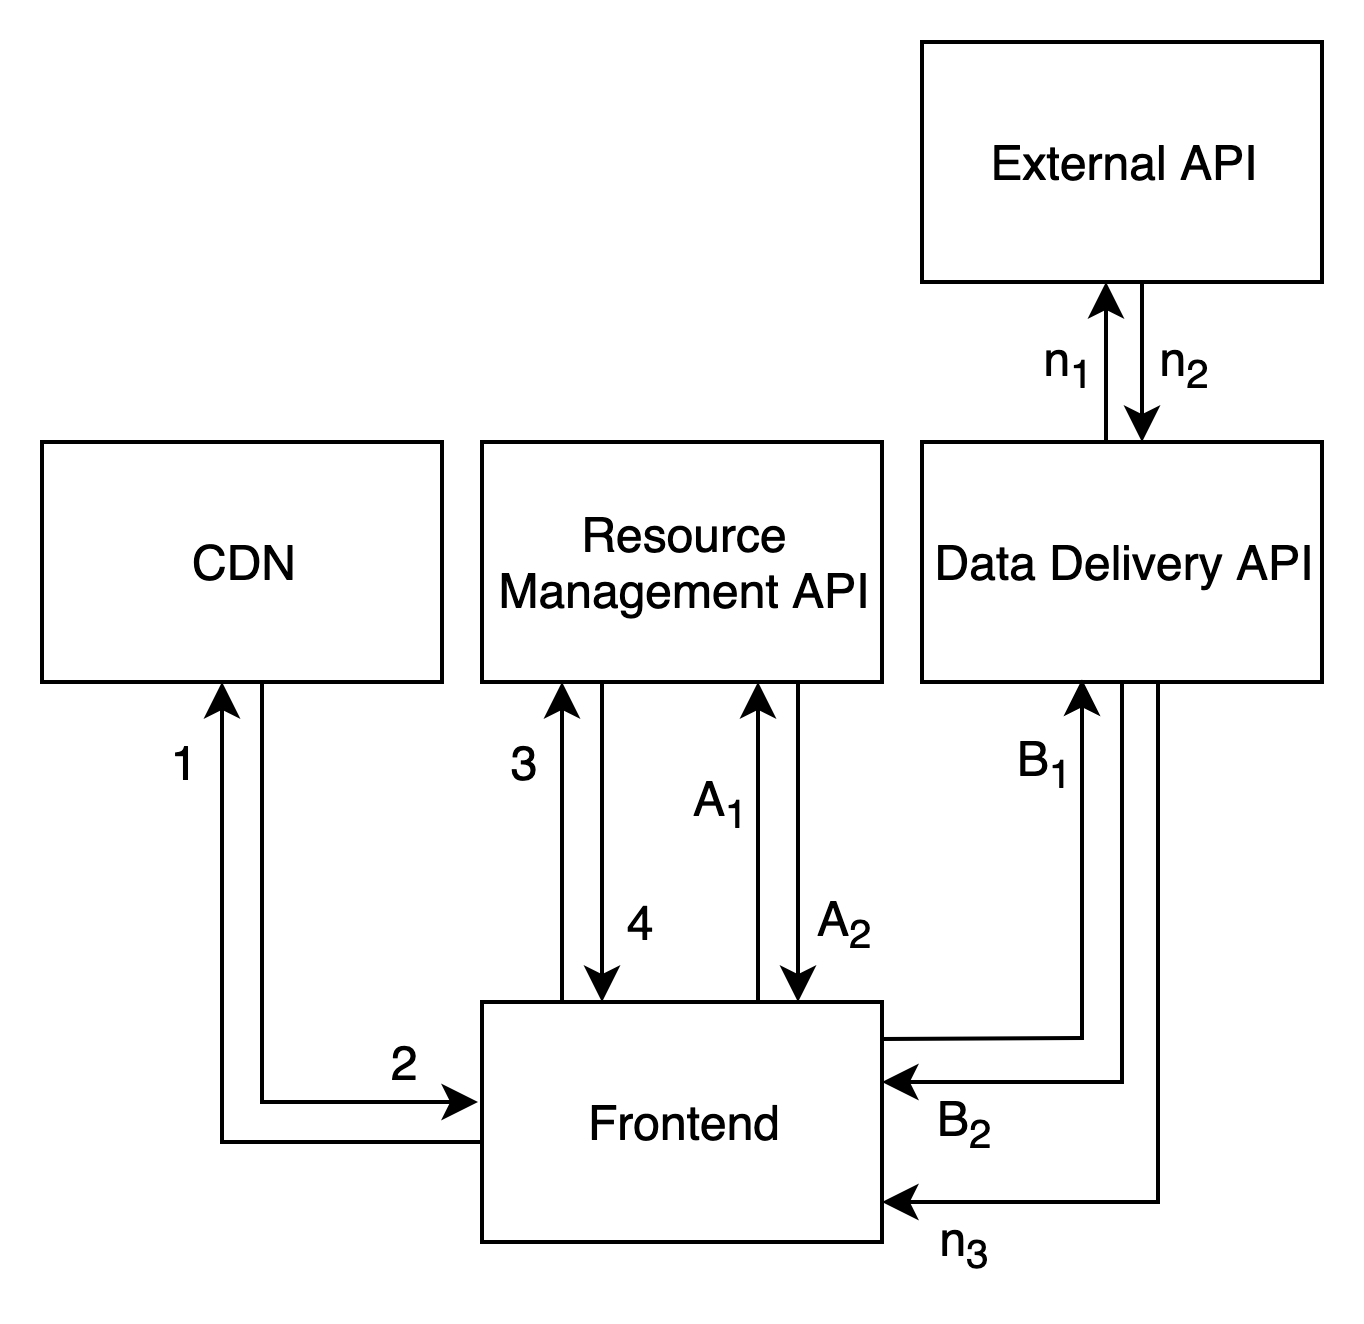
\includegraphics[scale=0.2]{img/abbildungen/InformationsaustauschDashboard}
    \end{center}
    \caption{Ablauf des Informationsaustausches eines Dashboards}
\end{figure}

\begin{figure}
    \label{figure:uebersichtderdatenauslieferung}
    \begin{center}
    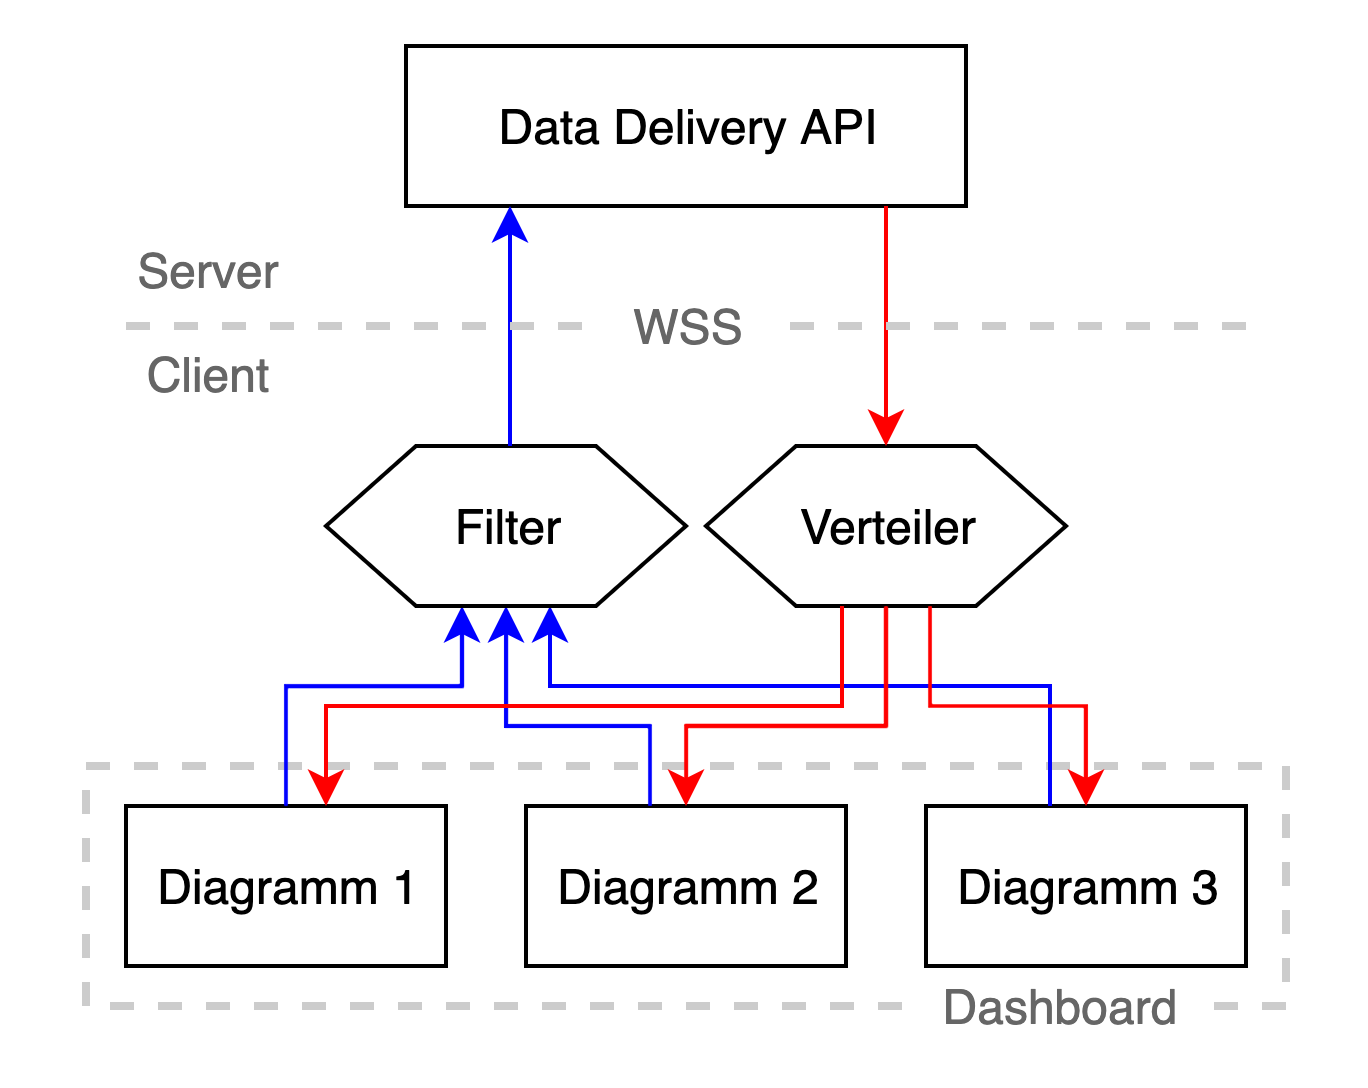
\includegraphics[scale=0.2]{img/abbildungen/Verteilung}
    \end{center}
    \caption{Verringerung der Redundanz des Datenflusses}
\end{figure}

\begin{figure}
    \label{figure:screenshotdeswebsocketdatenverkehrs}
    \begin{center}
    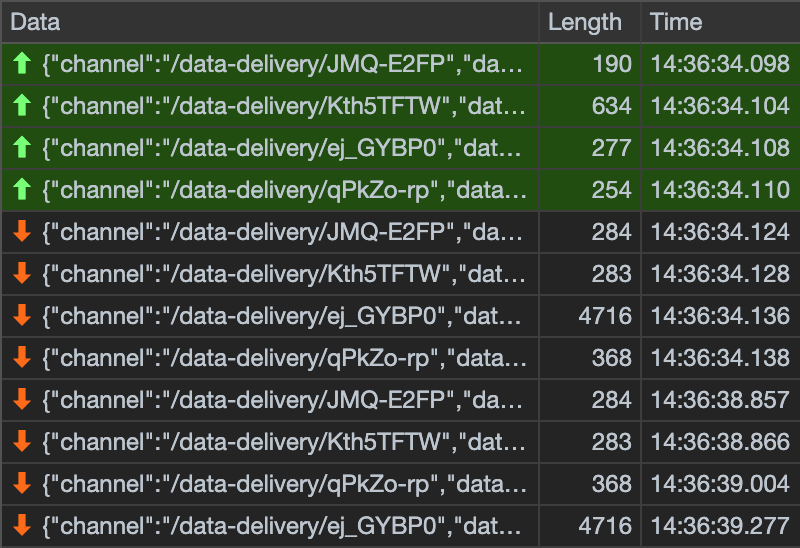
\includegraphics[scale=0.65]{img/screenshots/WebSocketTraffic}
    \end{center}
    \caption{Screenshot des WebSocket-Datenverkehrs}
\end{figure}
% Erkenntnis, Der Cache ist viel schneller, Cache ist O(1) wohingegen datenverarbeitung O(n) ist siehe
% anhand der größeren Anfrage

\subsection{WWS Handshake Authentifizierung}
\subsection{Golang MongoDB Aufbau}

\section{Plugins}
\subsection{Code Splitting und Lazy Loading}
% loading plugins on runtime
\subsection{D3.js und Chart.js}
\begin{listing}
    \label{lst:HelloJSX}
    \caption{Ein einfaches JSX Beispiel}
    \inputminted{jsx}{snippets/examples/Welcome.jsx}
\end{listing}

\begin{listing}
    \label{lst:Golang}
    \caption{Ein einfaches Golang Beispiel}
    \inputminted{go}{snippets/examples/hello.go}
\end{listing}
